\chapter{What is Blazon?}

Blazon is the language of heraldry and family crests. The language dates back to the twelfth century and provides a strict set of rules about how to produce a coat of arms.  
There are several different versions of Blazon found around Europe; however all follow the same behavioural rules regarding tinctures and charges.  Most versions differ only in the set of tinctures and honourable ordinaries by either having a more generous or conservative view on what is and isn't acceptable. For example, African Blazon allows for an orange coloured tincture whilst English Blazon does not.
For this project I focused on exclusively on a strict English Blazon.  


Blazon is a powerful language for allowing limitless combinations and configurations of patterns and shapes to be \emph{Blazoned} onto a shield in and recorded in a concise textual description.

What is impressive about the language is that it achieves flexibility whilst reaming fairly formal and well defined, 
restricting the set of tinctures to a total of seven while maintaining a low number of pre-defined,  honourable ordinaries. 

Blazon, like any other language, has some unique terminology used to address certain aspects of heraldry.  Anyone attempting to utilize the language will need to familiarise themselves with this terminology.    



\section{The Seven tinctures}
The most fundamental elements of Blazon are the tinctures.  Tinctures are comprised of a set of colours allowed in coats of arms.  English Blazon defines a set of seven tinctures and places them into to groups metals and colours. 

\begin{figure}[The Seven tinctures]
\centering
\begin{tabular}{| c | c | c |}

	\hline
	\multicolumn{3}{| c |}{The Seven tinctures} \\ \hline

	tincture & colour & metal/colour \\ \hline

	Azure & Blue & colour \\
	Argent & Silver & metal \\
	Gules & Red & colour \\
	Or & Gold & metal \\
	Purpure & Purple & colour \\ 
	Sable & Black & colour \\
	Vert & Green & colour \\
	\hline
\end{tabular}
\caption{Table of tinctures found in English Blazon, the corresponding colours and whether each tincture is or isn't a metal.}
\label{tab:label}
\end{figure}


Although at first, it may seem overly restrictive; Blazon overcomes having a limited set of valid tinctures by leaving interpretation of the tone and shade of each tincture's corresponding colour to the artist producing the shield. 
An Azure (blue) shield could be a light sky blue or a dark navy shade of blue depending upon the artists preference, as long as it is recognisably blue. 

The Freedom of Interpretation is a great attribute of Blazon which vastly increases the different graphical variations of Blazoned shields without radically increasing the size of the language. This is done by exhaustively listing a set of valid tones and shades. 

With regard to the two metallic tinctures Or, gold, and Argent, silver, having freedom of interpretation allows for matt, non-metallic, colours to be placed onto a shield, although they will still behave as metal tinctures.  It is not uncommon to see yellow instead of gold and white instead of silver on many coats of arms.


\section{Furs}

Blazon incorporates several furs commonly used in coats of arms.   These behave in much the same way as tinctures but don't have the same metal or colour property.

There are several pre-defined patterns for furs that are used directly instead of actual fur on a shield.  These patters generally consist of a repeating pattern on-top of a background colour.  Each fur has a unique pattern although several are very similar, some simply being the inverse of another.

The colours of Furs are pre-defined but can be explicitly stated as differing from the normal colours  by stating the tinctures to be used instead.  For example, Ermine coloured silver and black would be defined as \emph{"Ermine Argent and Sable"} 

% figure here showing furs please

\section{Fields}
A field is defined as an area on a shield.  Initially, a shield has one implicit field, which is the entire area of that shield.  Blazon allows for two operations on fields, a field can be tinctured, with a tincture or a Fur, or a field can be partitioned. 

Tincturing a field dictates that the whole area incorporated within that field be filled in the colour of that tincture.  Partitioning will covered in much more detail later on.



\section{How to Blazon a Coat of Arms: Part One}

A large enough subset of Blazon has now been defined for a couple of basic examples.  

Each example is implicitly provided with a single field which encompasses the entire body of the shield.  Then that field is tinctured by providing a Blazon sentence which includes a tincture.  This will successfully Blazon the shield.

\begin{figure}[H]
\subfigure[\emph{"Vert"}]{
\includegraphics[width=0.4\textwidth]{Blazon/images/vert.eps}}
\hfill
\subfigure[\emph{"Or"}]{
\includegraphics[width=0.4\textwidth]{Blazon/images/or.eps}}
\hfill
\subfigure[\emph{"Azure"}]{
\includegraphics[width=0.4\textwidth]{Blazon/images/azure.eps}}
\hfill
\subfigure[\emph{"Gules"}]{
\includegraphics[width=0.4\textwidth]{Blazon/images/gules.eps}}
\hfill
\caption{Basic Blazon examples.}
\label{Basic examples}
\end{figure}

Although the examples in Figure 2.1 are very basic, each is a complete instance of a valid Blazoning of a shield.







\section{Partitioning a field}
So far, the Blazon that has been introduced is very limited, only allowing for single tincture shields.  The next natural area of the language to define is the operation of Partitioning a field, which is a bit more complex and sophisticated.  

As stated previously, a field can be either tinctured or Partitioned.  To Partition a field the key-word \emph{"Per"} is used. It is obligatory that the word immediately after \emph{"Per"} is a type of partition.  Blazon has several pre-defined partitions, ranging from the very simple \emph{"Fess"}, which divides a field horizontally in half, to the more complex \emph{"Saltire"}, which divides a filed into four sections diagonally. 

Partitioning a field divides it up into several smaller fields.  The number and shapes of which depend on the type of Partition used.  After the Partition has been stated the Blazon sentence must go on to address the resulting new fields. 

A shield is implicitly Blazoned from top left to bottom right with the top most field taking priority. If two or more fields are adjacent at the same height, the left most takes priority.  

The Blazon sentence is only complete when all fields have been tinctured.  If a Blazon sentence Partitions a shield into two fields and provides only one tincture that sentence is invalid.  

% figures of all the partitions 



\begin{figure}[H]
\subfigure[\emph{"Fess"}]{
\includegraphics[width=0.5\textwidth]{Blazon/images/fess.eps}}
\hfill
\subfigure[\emph{"Pale"}]{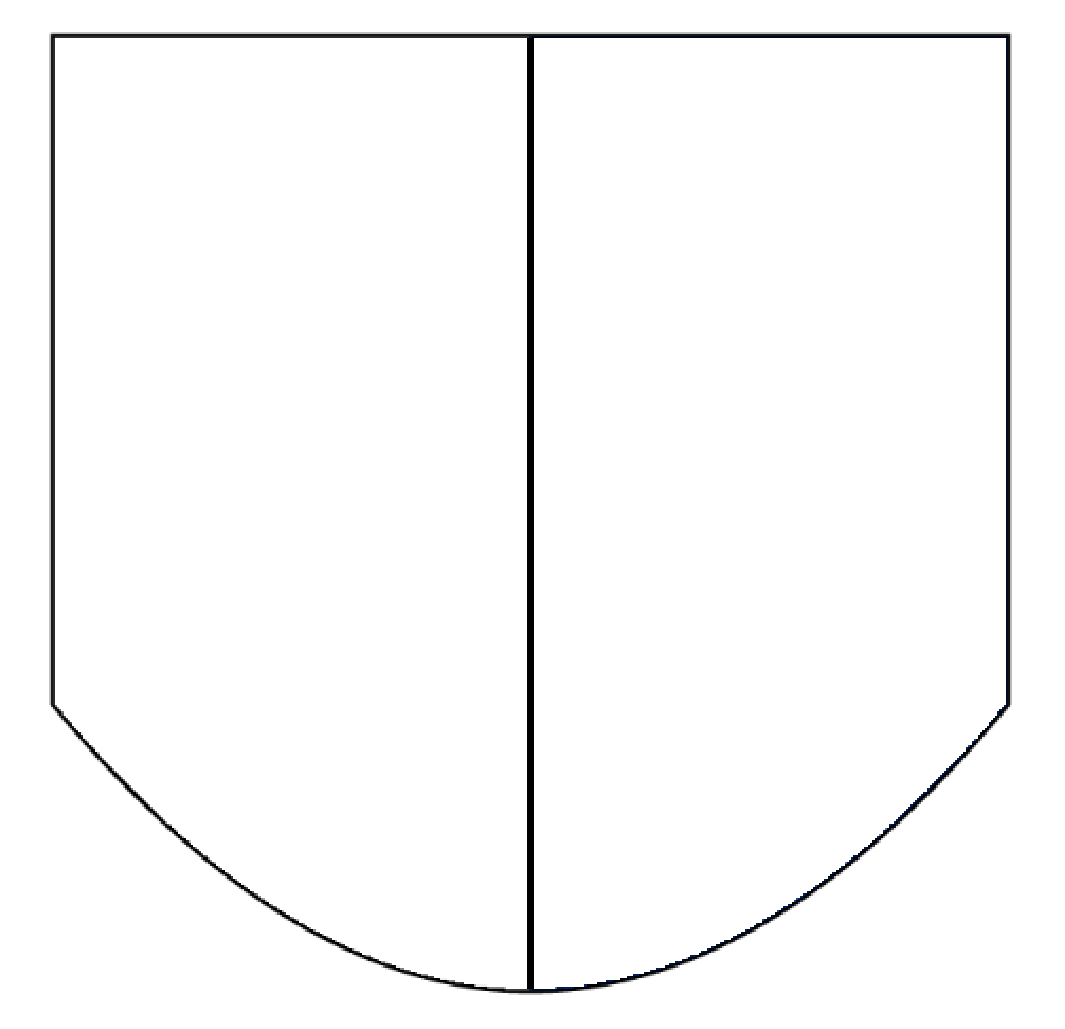
\includegraphics[width=0.5\textwidth]{Blazon/images/pale.eps}}
\hfill
\subfigure[\emph{"Bend"}]{
\includegraphics[width=0.5\textwidth]{Blazon/images/bend2.eps}}
\hfill
\subfigure[\emph{"Bend Sinister"}]{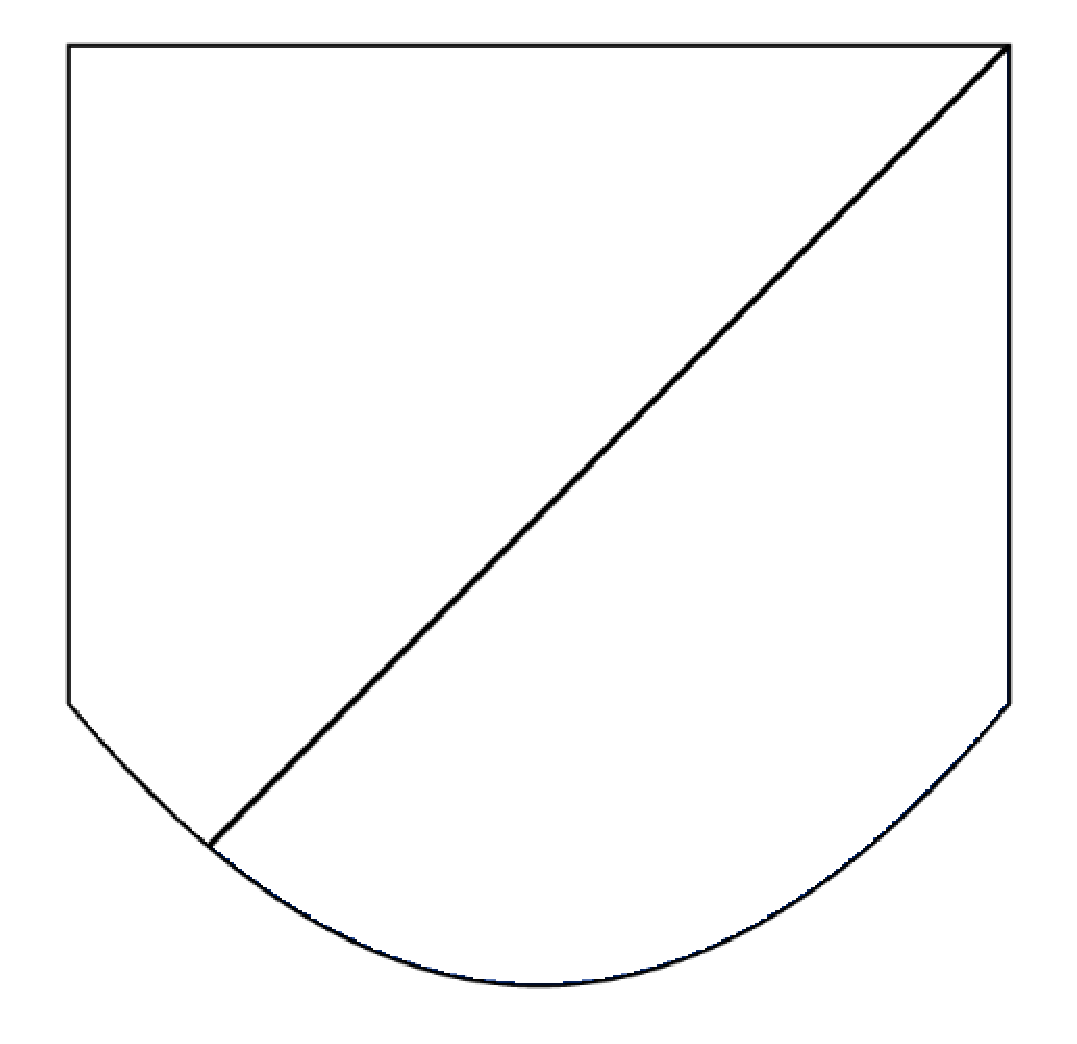
\includegraphics[width=0.5\textwidth]{Blazon/images/bendsinister.eps}}
\hfill
\end{figure}

\begin{figure}[H]
\subfigure[\emph{"Cheveron"}]{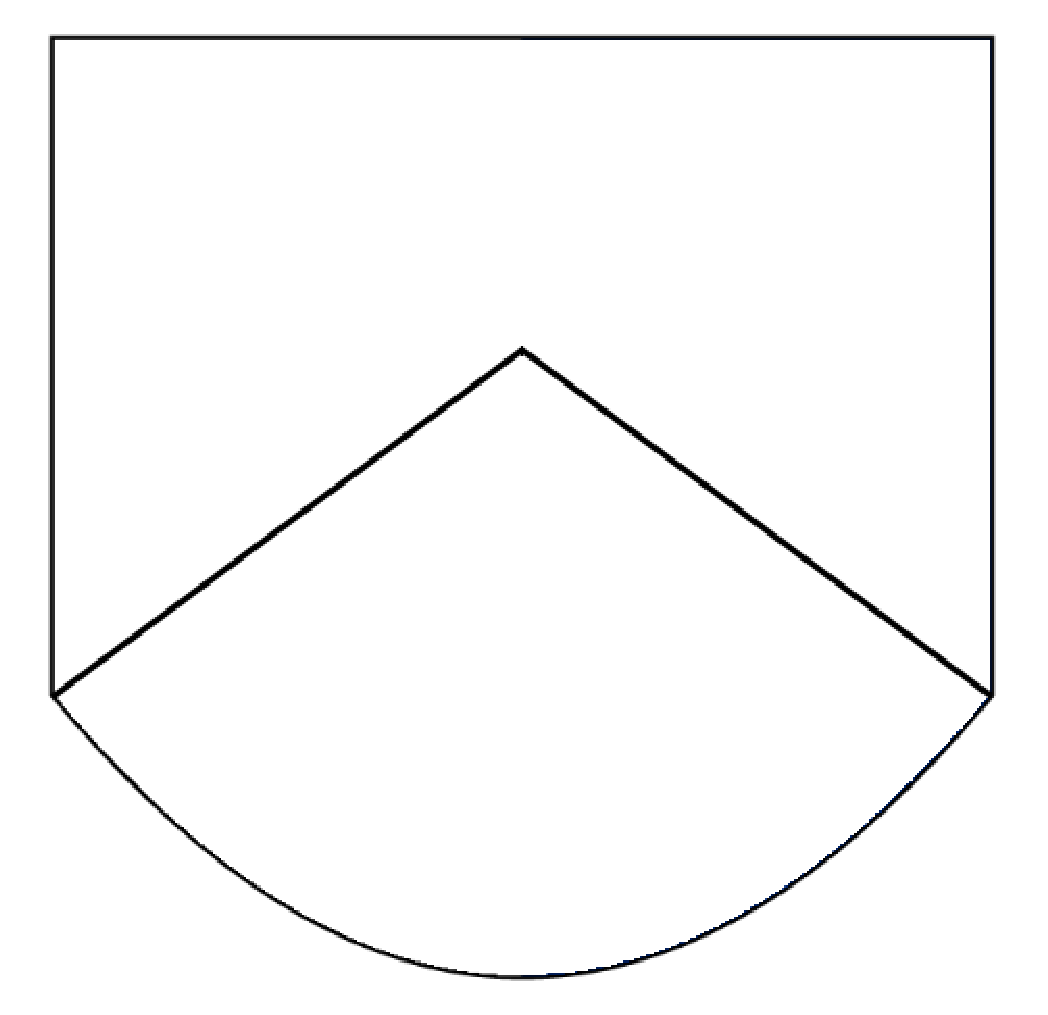
\includegraphics[width=0.5\textwidth]{Blazon/images/cheveron.eps}}
\hfill
\subfigure[\emph{"Pall"}]{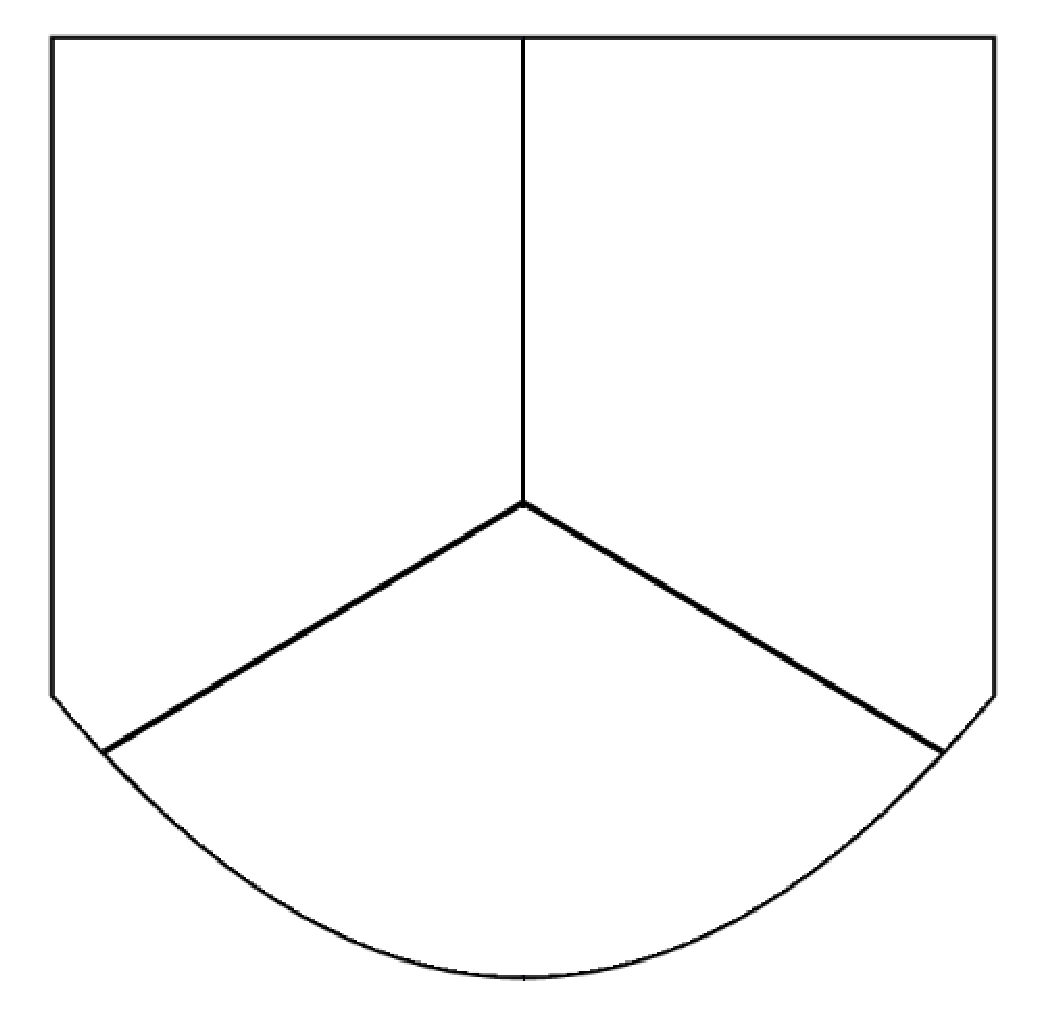
\includegraphics[width=0.5\textwidth]{Blazon/images/pall.eps}}
\hfill
\subfigure[\emph{"Cross"}]{
\includegraphics[width=0.5\textwidth]{Blazon/images/cross.eps}}
\hfill
\subfigure[\emph{"Saltire"}]{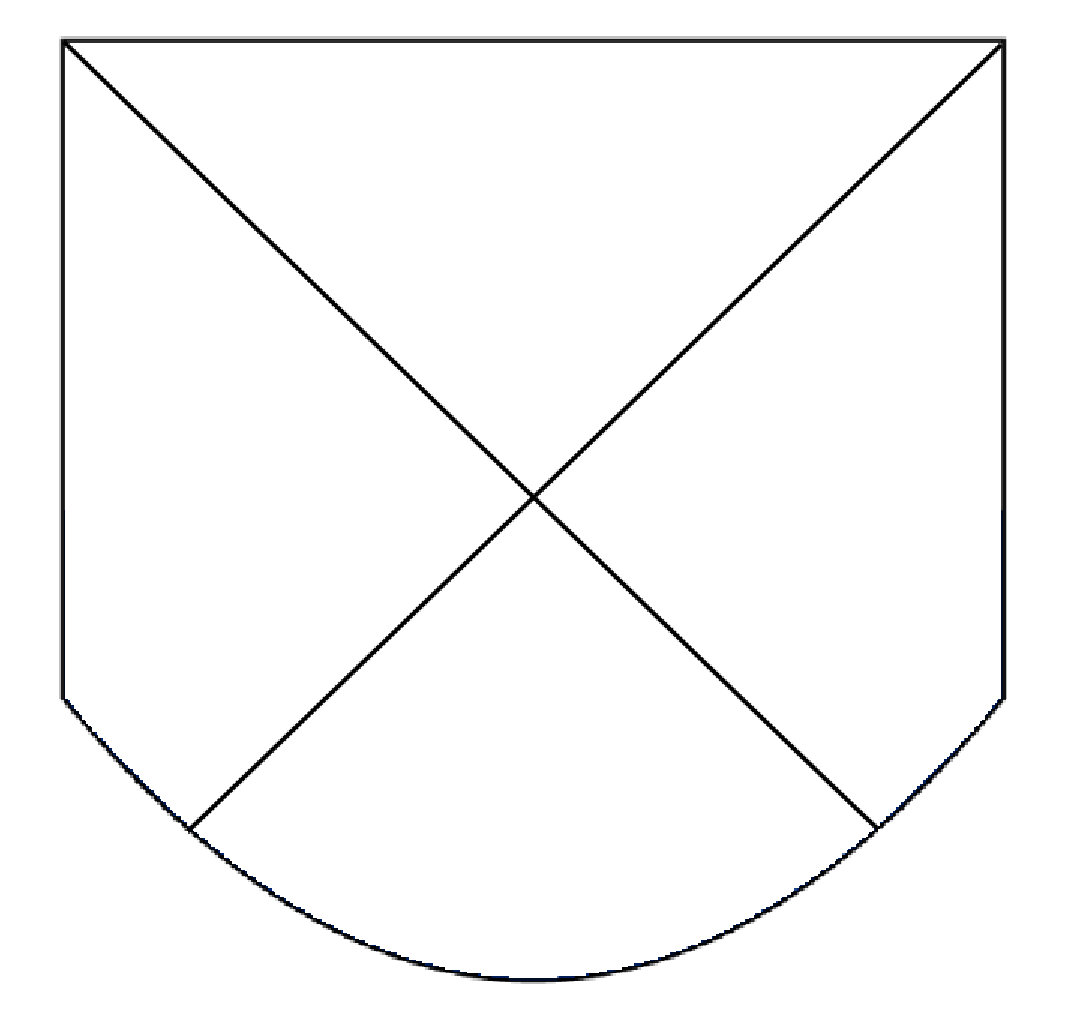
\includegraphics[width=0.5\textwidth]{Blazon/images/saltire.eps}}
\hfill

\caption{\emph{"Valid Partitions of a field"}}
\label{Partitions}

\end{figure}



\section{How to Blazon a Coat of Arms: Part Two}
Partitioning is a very powerful aspect of Blazon and increases the number of possible shield designs immensely.  A lot of very striking designs can be Blazoned onto a shield with very short Blazon sentences making use of partitioning.  


The Blazon sentence,\emph{"Per Bend Gules and Azure"} implicitly starts with a single field which encompasses the entire body of the shield. 


The implicit  field  is then partitioned into two smaller fields with the keyword \emph{"Per"} which declars a partition.  This is followed by the word \emph{"Bend"} which is a diagonal division of the field from top left to bottom right.

The Blazon sentence then goes on to tincture the two new fields with the tinctures \emph{"Gules"} and \emph{"Azure"} respectively.  Following Blazon's rule about evaluating the top-left most field first, the upper section of the shield is tinctured \emph{"Gules"} and then the lower half is tinctured \emph{"Azure"}.

After tincturing the fields, there are no more words remaining in the Blazon sentence and there are also no empty fields upon the shield. Therefore, this is a valid Blazon sentence and a striking red and blue shield has been produced. 


\begin{figure}[H]
\subfigure[\emph{"A single empty field."}]{
\includegraphics[width=0.4\textwidth]{Blazon/images/emptyfield.eps}}
\hfill
\subfigure[\emph{"The field has been partitioned Per Bend"}]{
\includegraphics[width=0.4\textwidth]{Blazon/images/bend.eps}}
\hfill
\subfigure[\emph{"The Topmost field is tinctured Gules"}]{
\includegraphics[width=0.4\textwidth]{Blazon/images/halfdoneperbendgulesandazure.eps}}
\hfill
\subfigure[\emph{"The final field is tinctured Azure"}]{
\includegraphics[width=0.4\textwidth]{Blazon/images/perbendgulesandazure.eps}}
\hfill
\caption{\emph{"Per Bend Gules and Azure"}.}
\end{figure}


By applying the same method as shown above, it is possible to validate the following Blazon sentences of similar complexity. 

\begin{figure}[H]
\subfigure[\emph{"Per Bend Sinister Argent and Vert."}]{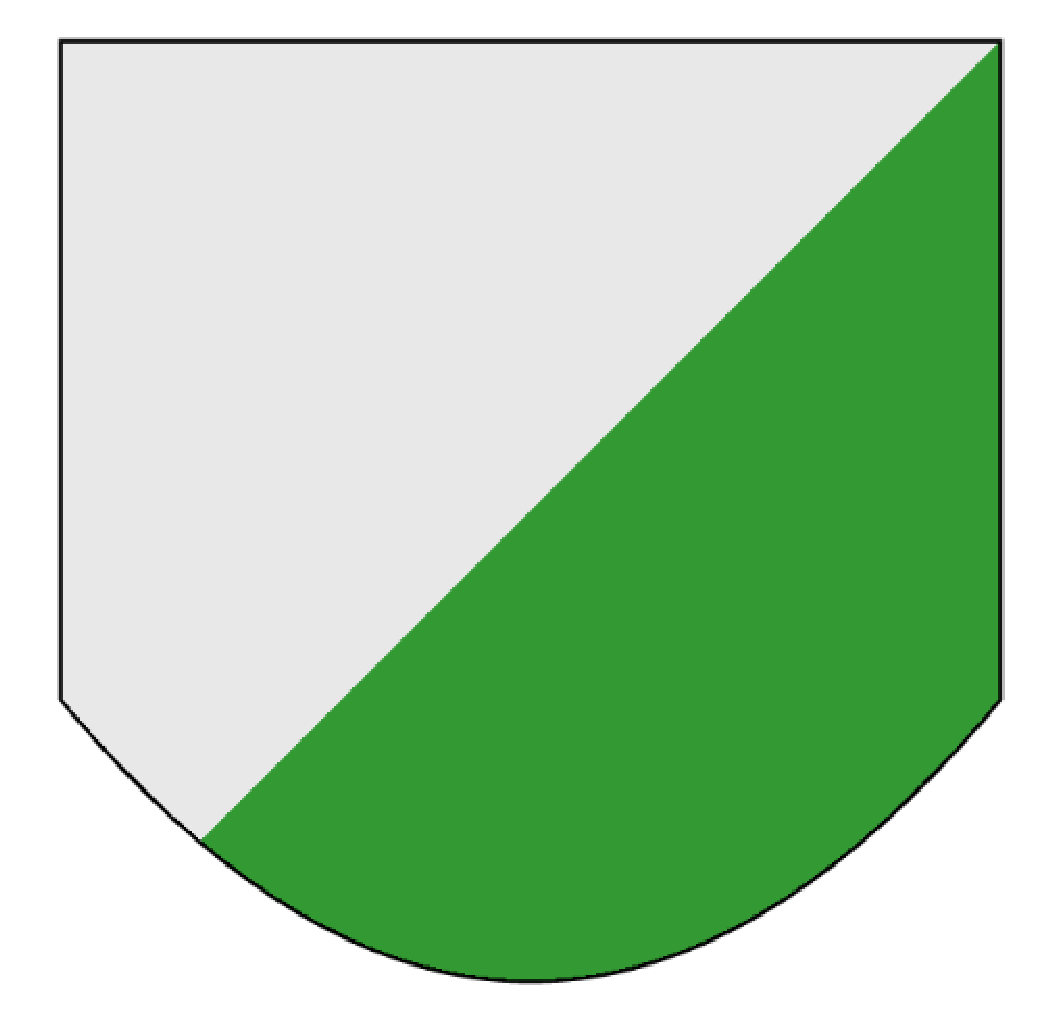
\includegraphics[width=0.4\textwidth]{Blazon/images/bendsinisterargentandvert.eps}}
\hfill
\subfigure[\emph{"Per Pale Azure and Or"}]{
\includegraphics[width=0.4\textwidth]{Blazon/images/perfessazureandor.eps}}
\hfill

\caption{\emph{"Two more examples of valid Blazon sentences"}.}
\end{figure}



\section{Sub-Partitioning}

The process of partitioning a field produces two or more smaller fields.  This allows for some very striking, though simple, designs.  Blazon allows for fields to be sub-partitioned where the new fields produced after a partitioning can themselves be partitioned. 

Considerably more advanced patterns can be achieved buy using sub-partitioning.  The complexity is potentially infinite as there is no limit enforced by the language as to how many partitions are allowed.  It is rare to see a historical shield Sub-Partitioned more than three times.  Sub-partitioning makes use of exactly the same set of partition types as regular partitioning.  

Sub-partitioning is expressed in exactly the same way as partitioning. When an  initial field has been partitioned instead of providing a tincture for one of the new fields, the keyword \emph{"Per"} is used to define a partition and then the type of partition is stated for example \emph{"Fess"}.  Each of the new fields need to be addressed either by being tinctured or further partitioned. 

The new fields created by the partition need to be fully evaluated before any other fields on the shield are addressed.  

New sub-fields are addressed according to the same rule present in regular Partitioning with the top-left most fields take priority.  Once all sub-fields have been evaluated, the next field according to partitioning rules is addressed.

\section{How to Blazon a Coat of Arms: Part Three}

With sub-partitioning, the set of valid Blazon sentences ceases to be finite.  It is possible to repeatedly partition a field then sub-partition the new sub-fields and endlessly repeating this process.  Very complex patterns can now be created with precisely defined sub-fields.

\emph{"Per Bend Per Pale Sable and Argent Per Fess Or and Gules"} is an example a Blazon sentence which makes use of sub-partitioning.  As before,  the sentence is addressed from left to right and there is an implicit field over the entire body of the shield.  The sentence is valid if there are as many fields defined as there are instances of tinctures in the sentence. 


\begin{figure}[H]
\subfigure[\emph{"A single empty field."}]{
\includegraphics[width=0.5\textwidth]{Blazon/images/emptyfield.eps}}
\hfill
\subfigure[\emph{"The field has been partitioned Per Bend"}]{
\includegraphics[width=0.5\textwidth]{Blazon/images/bend.eps}}
\hfill
\end{figure}

\begin{figure}[H]
\subfigure[\emph{"The Topmost field has then been Sub partitioned Pale"}]{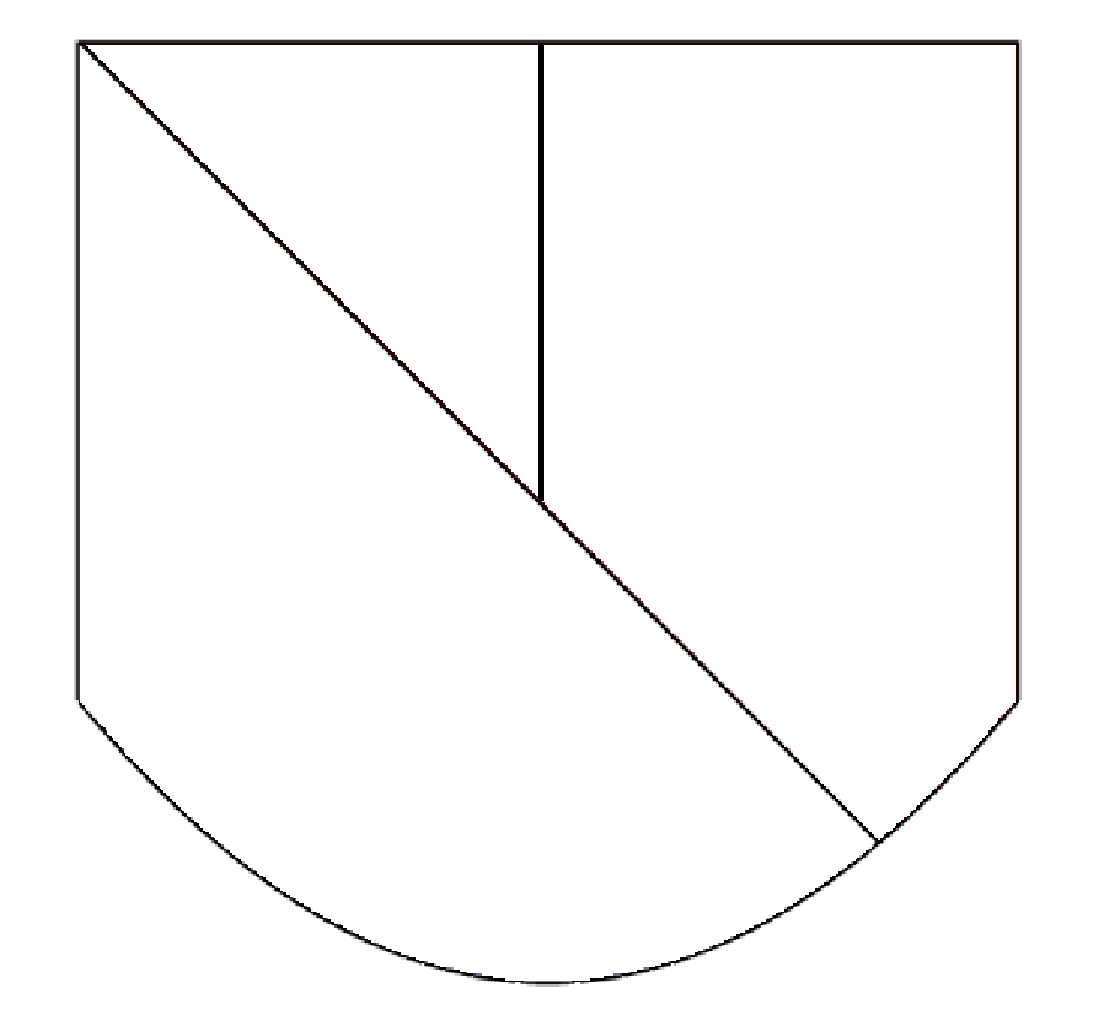
\includegraphics[width=0.5\textwidth]{Blazon/images/subpartition4.eps}}
\hfill
\subfigure[\emph{"The Top Left most Sub-field is tinctured Sable"}]{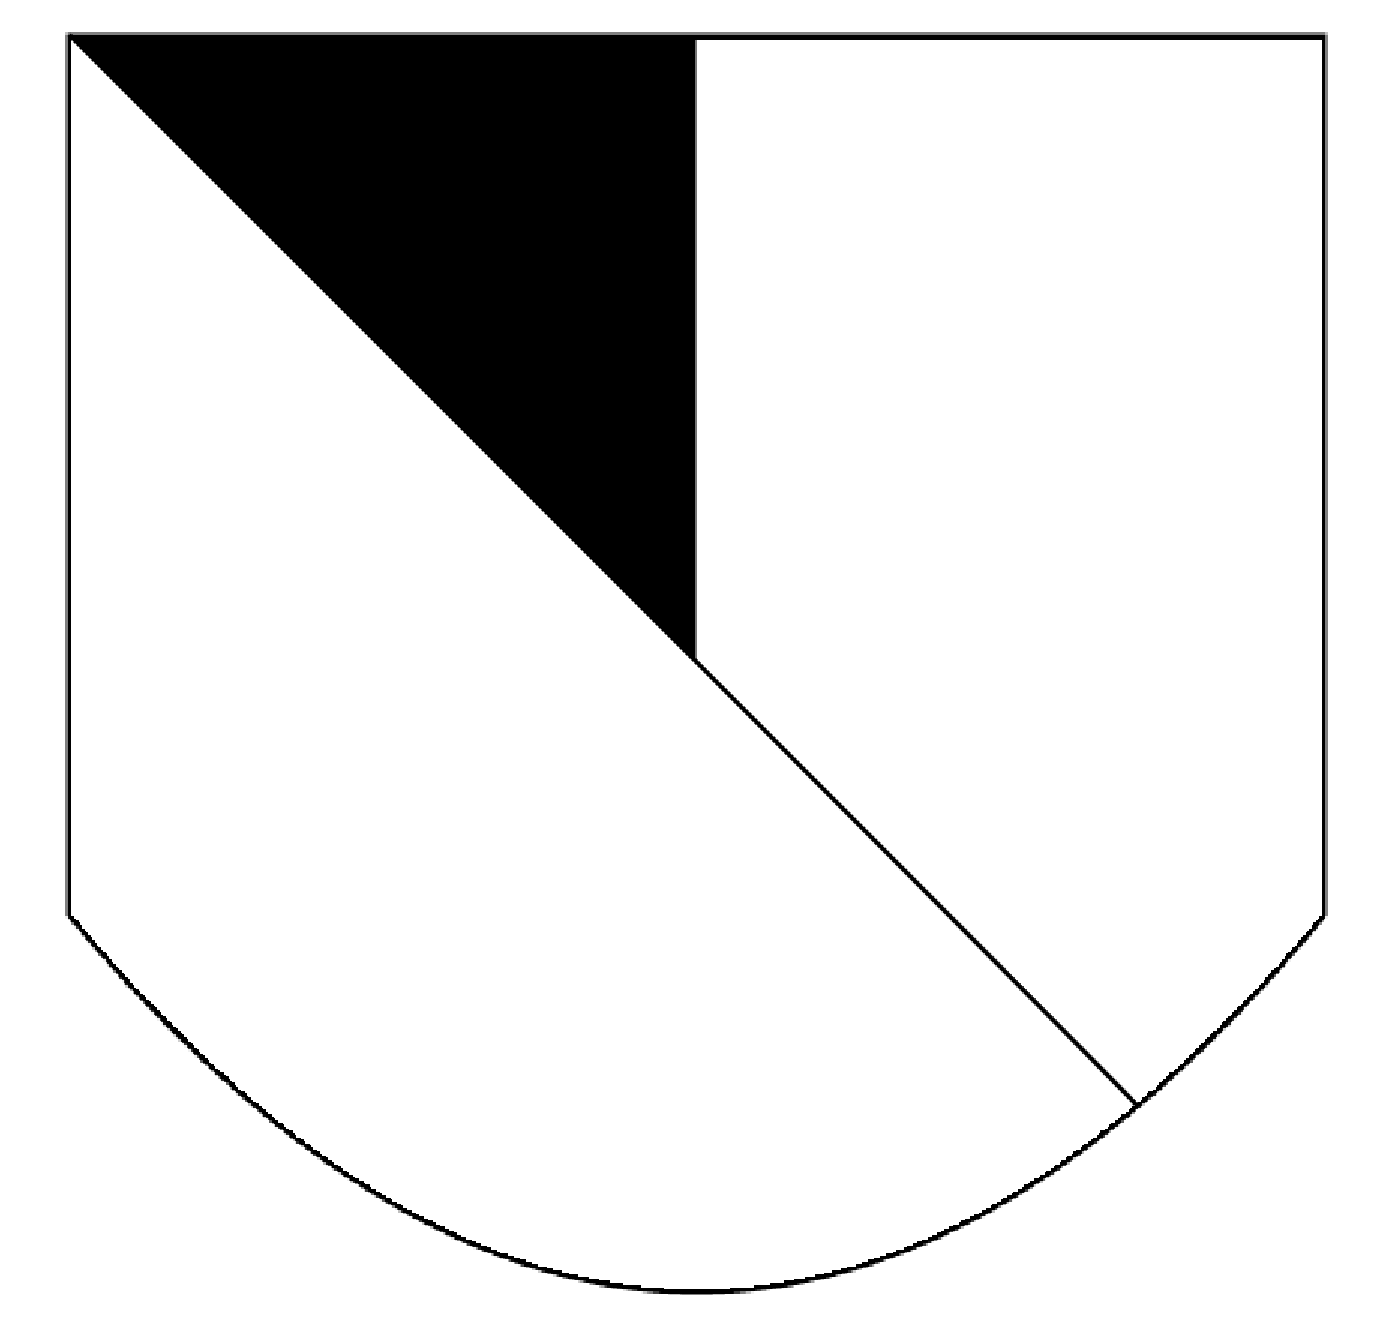
\includegraphics[width=0.5\textwidth]{Blazon/images/subpartition5.eps}}
\hfill
\end{figure}

\begin{figure}[H]
\subfigure[\emph{"The remaining field is Sub-Partitioned Fess"}]{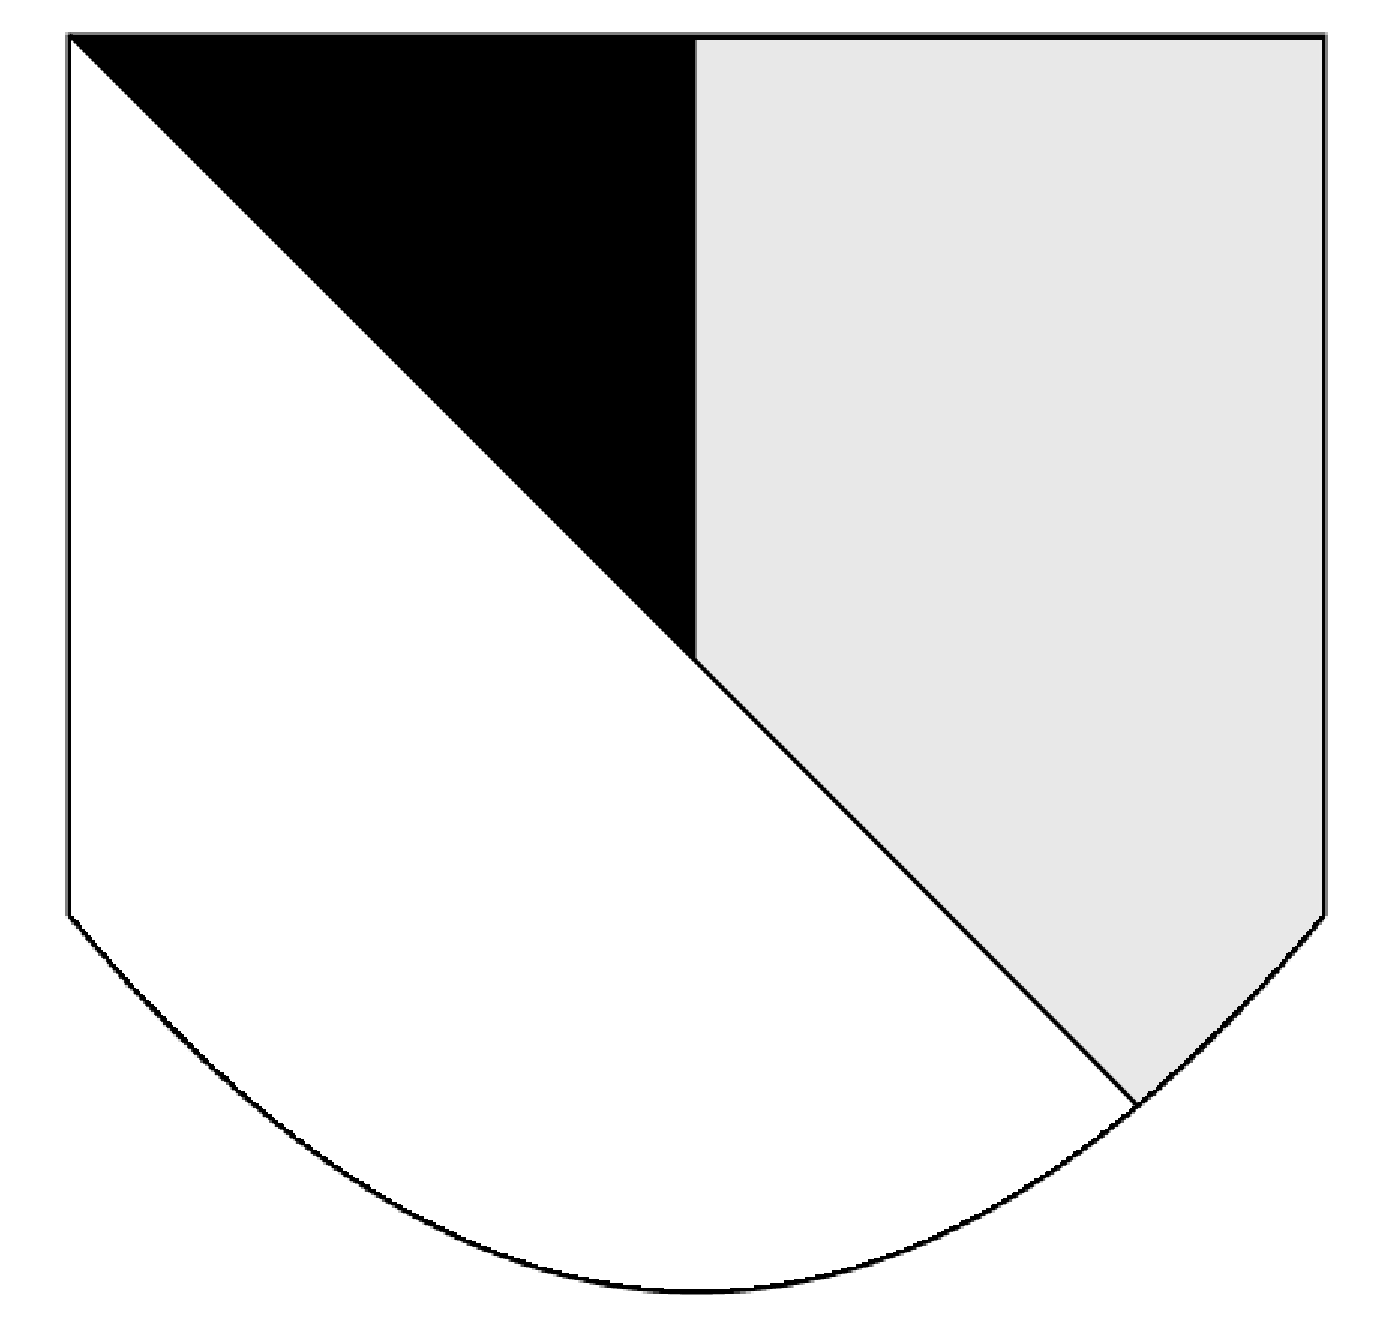
\includegraphics[width=0.5\textwidth]{Blazon/images/subpartition6.eps}}
\hfill
\subfigure[\emph{"The Top Left Most Sub-field is tinctured Or"}]{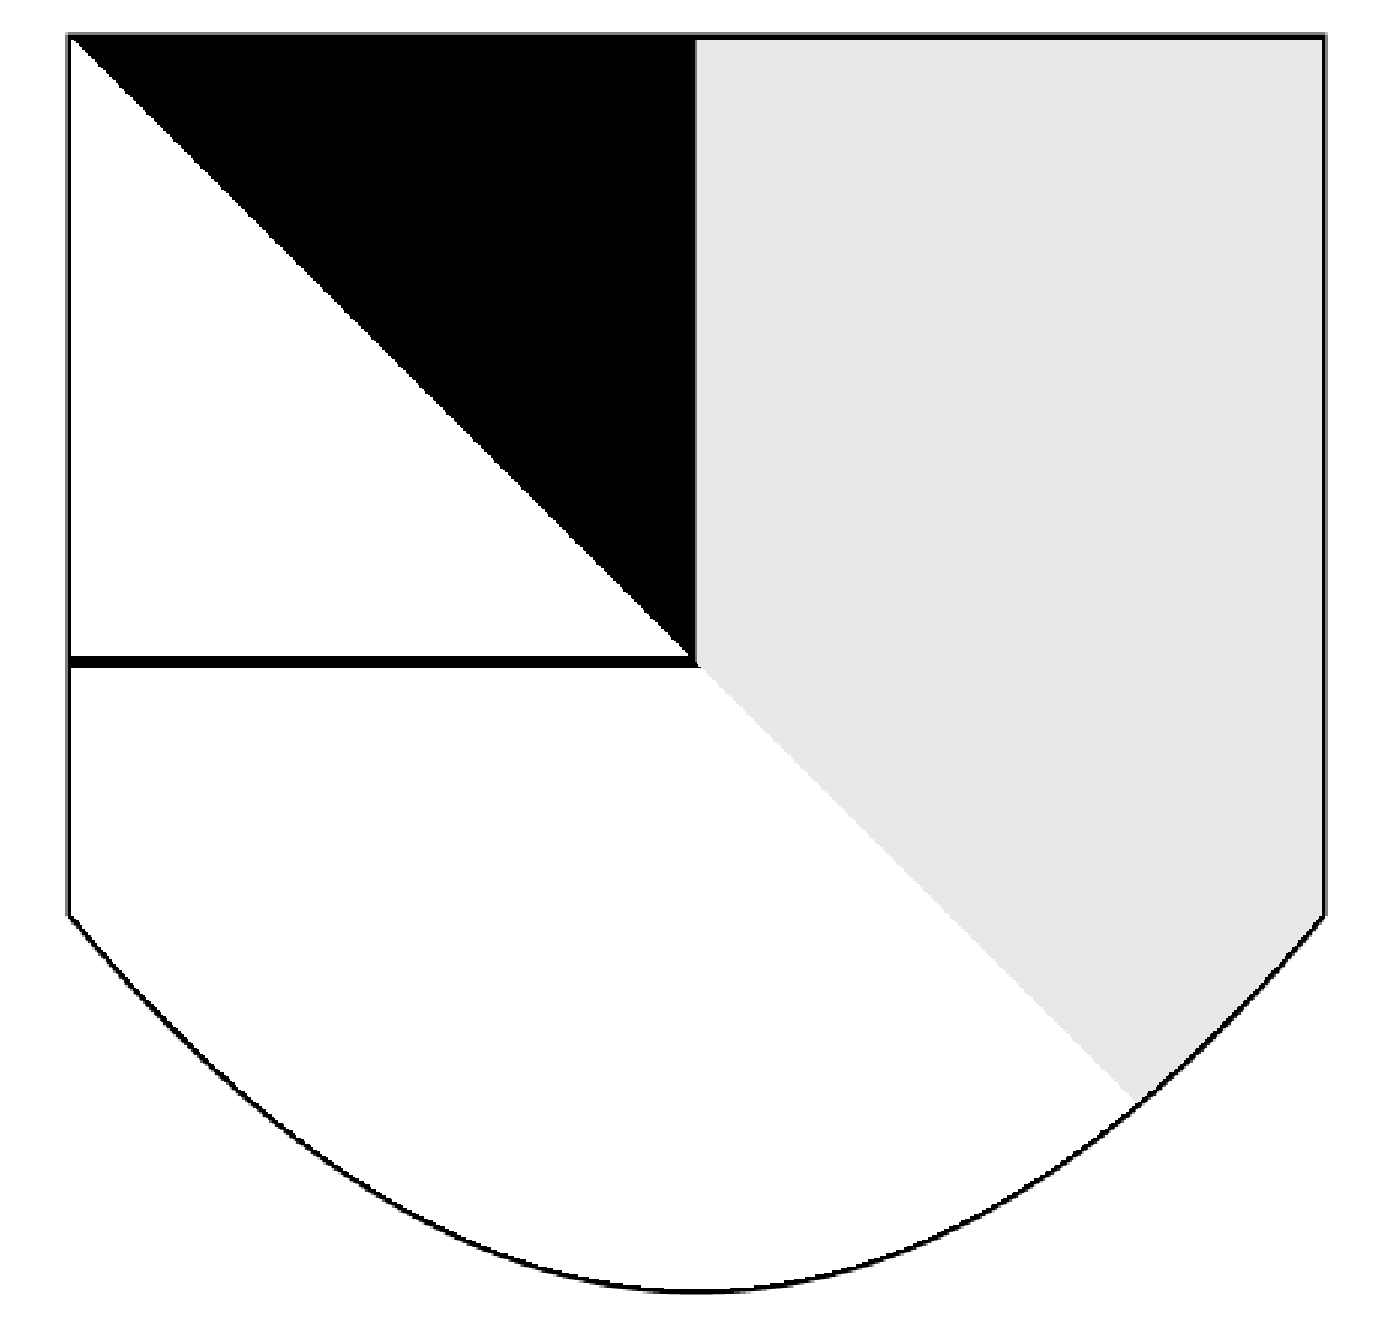
\includegraphics[width=0.5\textwidth]{Blazon/images/subpartition7.eps}}
\hfill
\end{figure}

\begin{figure}[H]
\subfigure[\emph{"The remaining Sub-field is Sub-Partitioned Fess"}]{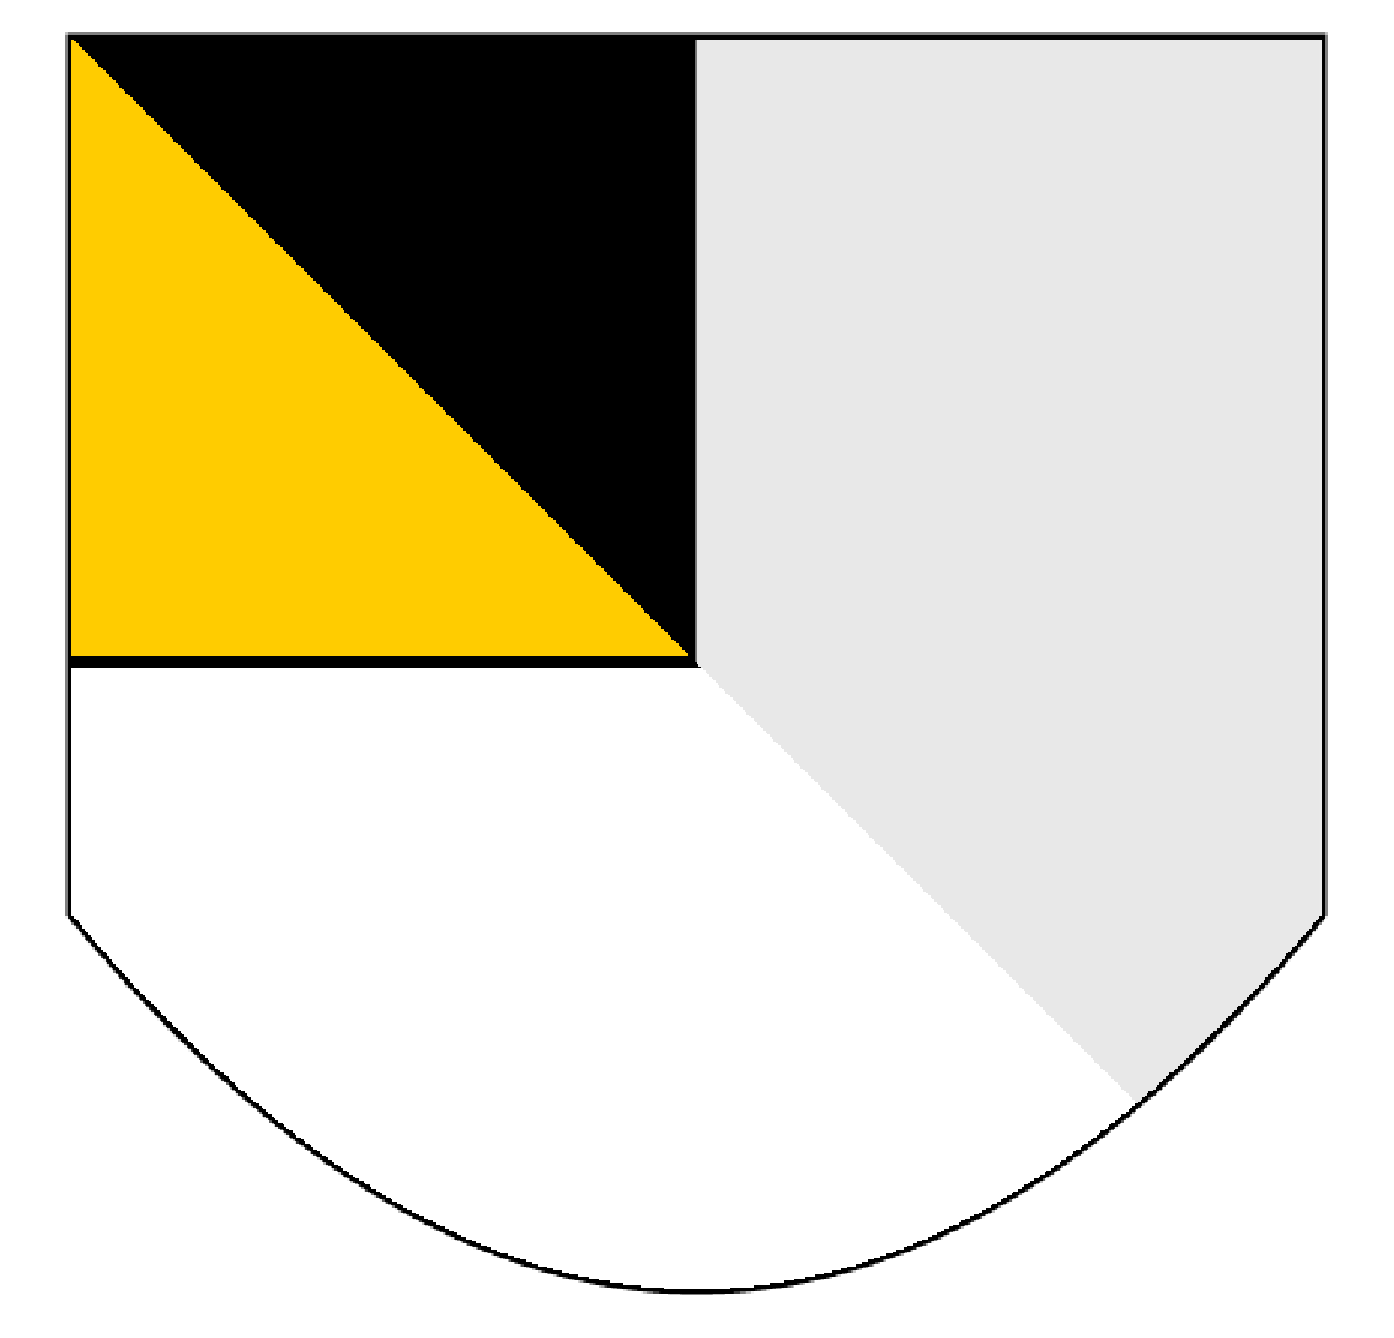
\includegraphics[width=0.5\textwidth]{Blazon/images/subpartition8.eps}}
\hfill
\subfigure[\emph{"The final field is tinctured Gules"}]{
\includegraphics[width=0.5\textwidth]{Blazon/images/perbendperpalesableandargentperfessorandgules.eps}}
\hfill
\caption{\emph{"Per Bend Per Pale Sable and Argent Per Fess Or and Gules"}.}
\end{figure}

\section{Line Types}

Blazon allows for partitions to be patterned with different line types.  The line division through a field when partitioning is implicitly straight; however, there are a set of pre-defined line types which can be used instead.  

A line type is declared in Blazon simply by stating the name of the line type desired immediately after a partition. For example, \emph{Per Fess Embattled Argent and Sable}, is the Blazon sentence for a silver and black shield divided horizontally with an \emph{"Embattled"} line, see Figure \ref{fig:lines}.  

Line types can be applied to sub-partitions and its possible to have multiple line types in a single Blazon sentence. 

\begin{figure}[H]
  \centering
    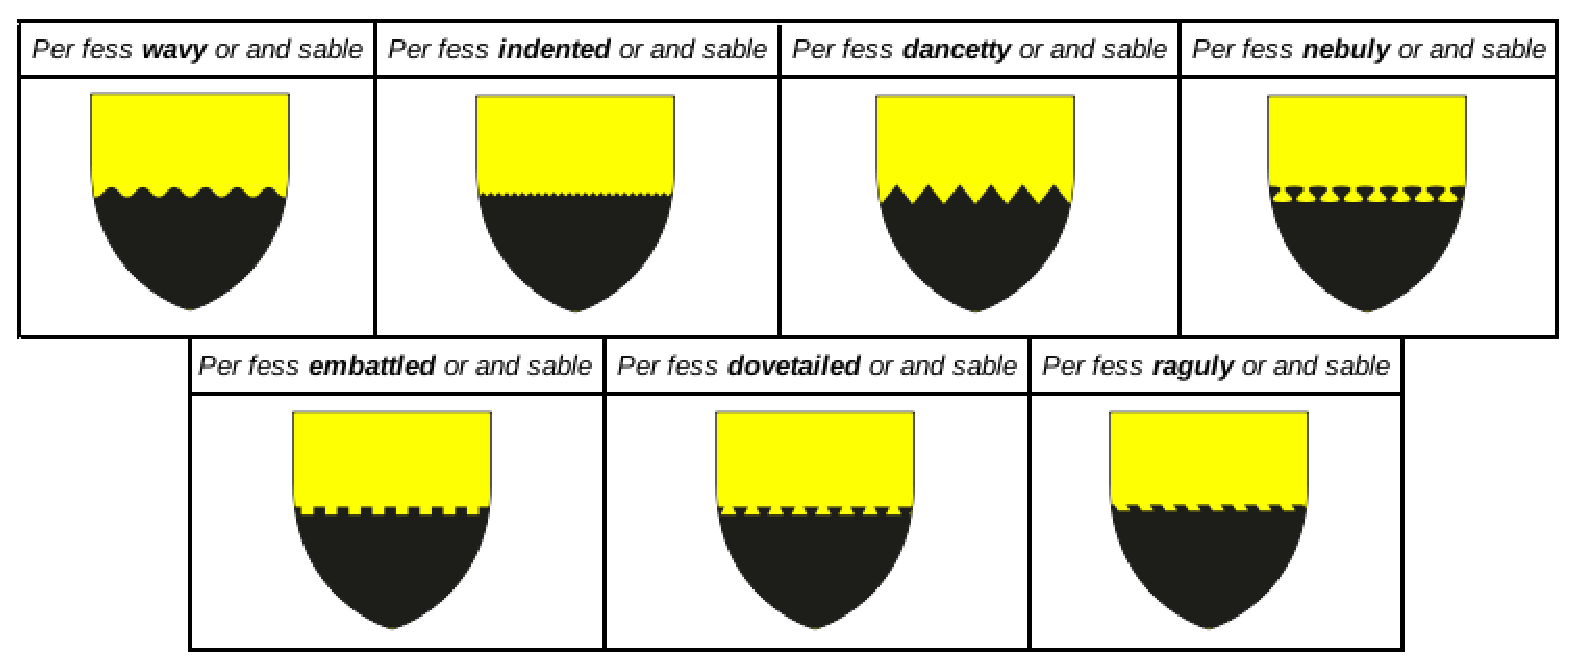
\includegraphics[width=\textwidth]{Blazon/images/linetypes.eps}
  \caption{Different line types valid in Blazon.\cite{linetypes}}
  \label{fig:lines}
  
\end{figure}


\section{Charges}
Another powerful aspect of Blazon is the ability to place pictures, called charges, onto a shield.  Charges can be placed onto any field that has been tinctured.  There are three subsets of charge, the honourable charges, the geometric charges and semi-formal charges.

The geometric charges are the most simple, consisting of a set of basic shapes such as a square and a circle.  The honourable charges are a set of predefined simple shapes some of which take after the partitions, such as \emph{"Bend"}.  The set of semi-formal charges contains everything that can be described textually.  Common examples are lions and eagles some royal Blazons have a crown as a charge. 


A charge is declared in a field by using a quantifier immediately after the field has been tinctured.  The quantifier is a pre-fix to the charge and determines how many instances of this charge are present on this field.  For example the sentence \emph{"Vert a Crown Or"} takes the implicit field then tinctures it \emph{Vert} before charging the field with a crown tinctured \emph{Or}, this would produce a green shield with a gold crown on it. Semi-formal charges can be tinctured \emph{"Proper"} which is their natural colours.  Even if a charge is a fictional creature, it will have a proper colouring.  Dragons are green when tinctured \emph{"Proper"}. 

The size and position of a charge is defined so that a charge should take up as much space as possible without obscuring any other charge or intersecting the perimeter of the field it is being placed onto.  

Its possible to have several instances of the same charge on a field. There are common ways to position such groupings of charges however there is freedom for the artist to arrange groups of charges differently.

A very wide but short field would better suit its charges being placed in a straight line rather than the usual grouping as long as each charge is visible. 


The prefix quantifier can be a number or amount to define how many types of this charge are present in field, \emph{Argent three Delfs Sable} would produce a silver shield with three black squares on it in a triangular pattern, one each in the  top corners and one centrally placed in toward the bottom. 

It is even possible to have multiple groupings of different Charges on a field for each charge. The grouping is treated individually so that it is not allowed to obscure any other charge.  

There are keywords which exist for specifying the position of Charges. For example,  \emph{"Beneath"} and \emph{"Above"}.  Keywords make it possible to position charges relative to other charges.

Finally, it is possible to place charges upon other charges.  This can be done with the keywords \emph{"in"} or \emph{"upon"}. For example, \emph{"Vert a Bend Azure upon a Chief Argent"} would produce a green shield with a silver bar along the top which has a blue diagonal bar on top of it.

\section{Attitudes}
Blazon allows semi-formal charges to be given an \emph{Attitude} to add further description to the charge.  This normally takes the form of an adjective applied as a suffix.  For example, a lion can be described as rampant or as passant both of which alter the pose the lion will be depicted in.  A lion rampant is depicted as rearing up on its hind legs with its claws raised; while a lion passant is standing horizontally with a single claw raised. 

%diagrams 

\begin{figure}[H]
\subfigure[\emph{"A Lion Rampant.\cite{rampant}"}]{
\includegraphics[width=0.5\textwidth]{Blazon/images/rampant.eps}}
\hfill
\subfigure[\emph{"A Lion Passant"\cite{passant}}]{
\includegraphics[width=0.5\textwidth]{Blazon/images/passant.eps}}
\hfill
\caption{\emph{"An example of applying attitudes to a charge"}.}

\end{figure}



\section{The Rule of tincture}
One of the most important and widely followed rules of Blazon is the rule of tincture which states that \emph{a colour may not be placed upon a colour nor a metal be placed upon a metal}\cite[p.46]{ruleoftincture}.  This rule makes certain tincture combinations of charges and fields invalid with each other.  As stated above in \ref{tab:label}, every tincture is either a metal or a colour in accordance with the Rule of tincture, a Charge tinctured with a colour can only be placed upon a field tinctured with a metal.  Likewise, A Charge tinctured with a metal can only be placed upon a fields tinctured with a colour.  

Therefore, \emph{"Azure a Cross Gules"} is an invalid Blazon sentence because both Azure and Gules are colours and having a colour Charged upon another colour breaks the Rule of tincture.  The Rule also applies to Charges placed on Charges. 





\section{How to Blazon a Coat of Arms: Part Four}

Charges are equally as important in Blazon as Partitioning, they allow the language a freedom to have any object placed upon them. With this extra functionality comes a slightly more complex terminology as described above with new keywords and the need to observe the Rule of tincture.  

Taking, \emph{"Per Pale Azure a Cross Argent and Or a Saltire Gules"} as an example of a Blazon sentence which uses charges it is possible to demonstrate how Charges are used in Blazon.  

Starting with the implicit initial field the Blazon sentence starts \emph{"Per Pale"} which Partitions the field Per-wards, vertically. The left hand field is then addressed as it is the Top-Left most field not yet tinctured, the next word in the Sentence is a tincture \emph{"Azure"} which indicates this field is to be blue.  The next word in the sentence is \emph{"a"} which is a quantifier for a single charge which the Sentence states is a \emph{"Cross"} because the Charge is on a field which has been tinctured with a colour, the Charge must be a metal for the Blazon to be valid in this case the tincture is \emph{"Argent"} which is indeed a metal.  

As the next word of interest in the Blazon sentence is \emph{"Or"} which as a tincture and there have been no more charges declared we address the next field so the right half of the shield should be gold in colour. Then there is another qualifier again its \emph{"a"} indicating a single Charge which is stated as being a \emph{"Saltire"} tinctured \emph{"Gules"} this produces a colour Charge on a metal field and thus respects the Rule of tincture.  

There are no more words remaining in the Blazon sentence, all the fields and Charges have been tinctured and the Rule of tincture has not been broken, therefore, \emph{"Per Pale Azure a Cross Argent and Or a Saltire Gules"} is a valid Blazon sentence which contains two fields each with a single Charge. 


%diagrams please

\begin{figure}[H]
  \centering
    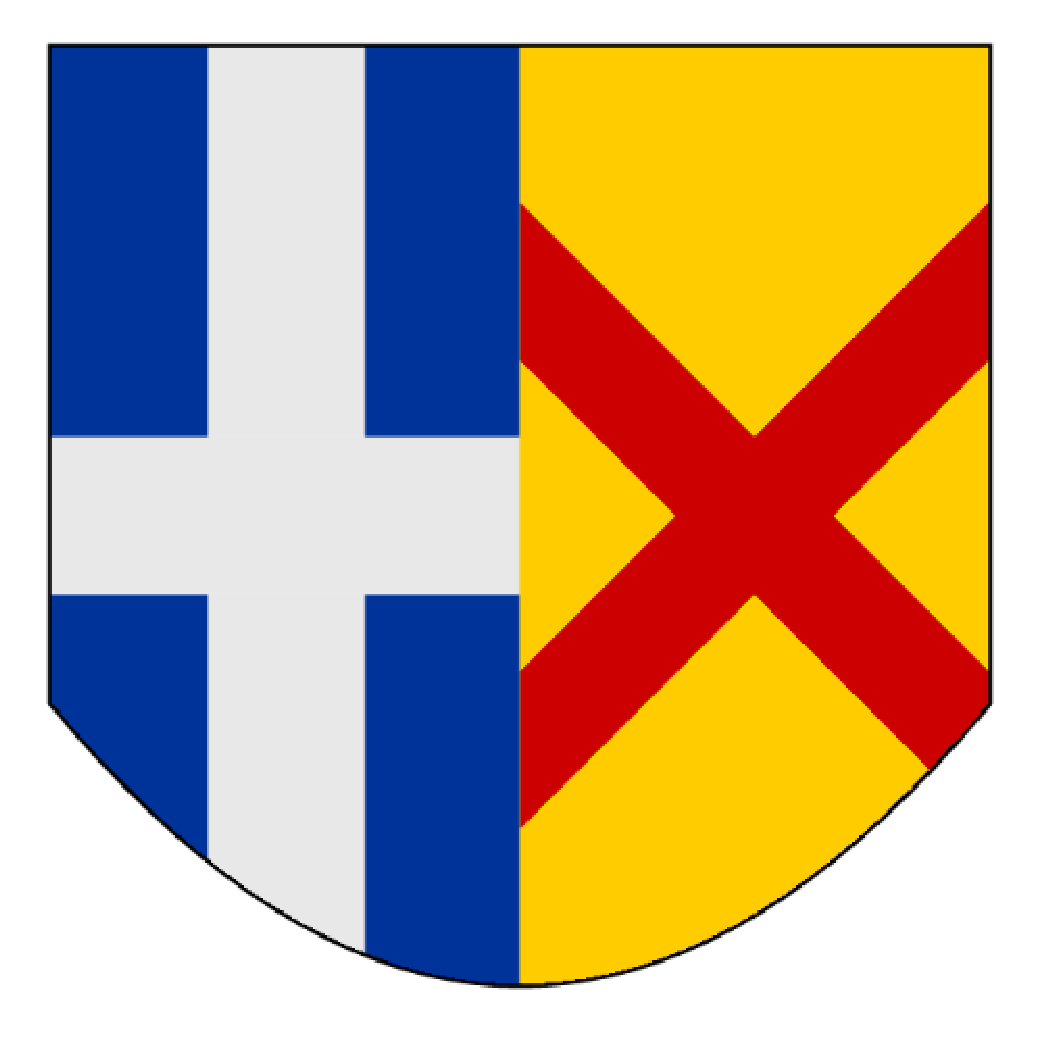
\includegraphics[width=\textwidth]{Blazon/images/perpaleazureacrossargent.eps}
  \caption{\emph{"Per Pale Azure a Cross Argent and Or a Saltire Gules"}.}
  
\end{figure}

\section{Counter-Charging}

Blazon also provides functionality for positioning Charges across fields; this is achieved though \emph{Counter-Charging}.  If a Blazon sentence has two adjacent fields, then a Charge can be Counter-Charged across the two fields, this would split the charge down the line of Partition between the fields before Tincturing each half of the Charge inversely to the field it lies in.  Counter-Charging is performed using the keywords \emph{Counter Charged} as a suffix operator to a charge and must have two tinctured fields defined before it. 

In the example shown in figure \ref{fig:counter}
, the Blazon sentence for the shield defines a field Partitioned \emph{"Per Pale"} then the two resulting fields are tinctured \emph{"Argent"} and \emph{"Gules"} then a Charge is defined \emph{"a Bend"} which places a single diagonal bar upon the field then the keywords \emph{Counter Charged} are supplied instead of a tincture which extends the bar across the two fields and colours the section on the \emph{Argent} field in \emph{Gules} and the section on the \emph{Gules} field in \emph{Argent}.


\begin{figure}[H]
  \centering
    
\includegraphics[width=0.4\textwidth]{Blazon/images/countercharged.eps}
  \caption{\emph{"Per Pale Argent and Gules a Bend Counter Charged."\cite{countercharge}}}
  \label{fig:counter}
  
\end{figure}

\section{Directions and Sides}
The Blazon language contains a set of words for describing positions and directions.  These words are obviously useful for more accurately placing Charges on a field.  The top of the shield is refereed to as \emph{Chief} and the bottom is refereed to as \emph{Base}.  The Left hand side of the shield, from the viewers perspective is called to as \emph{Dexter} and the right hand side, again from the views perspective, is \emph{Sinister}. 

\begin{figure}[H]
  \centering
    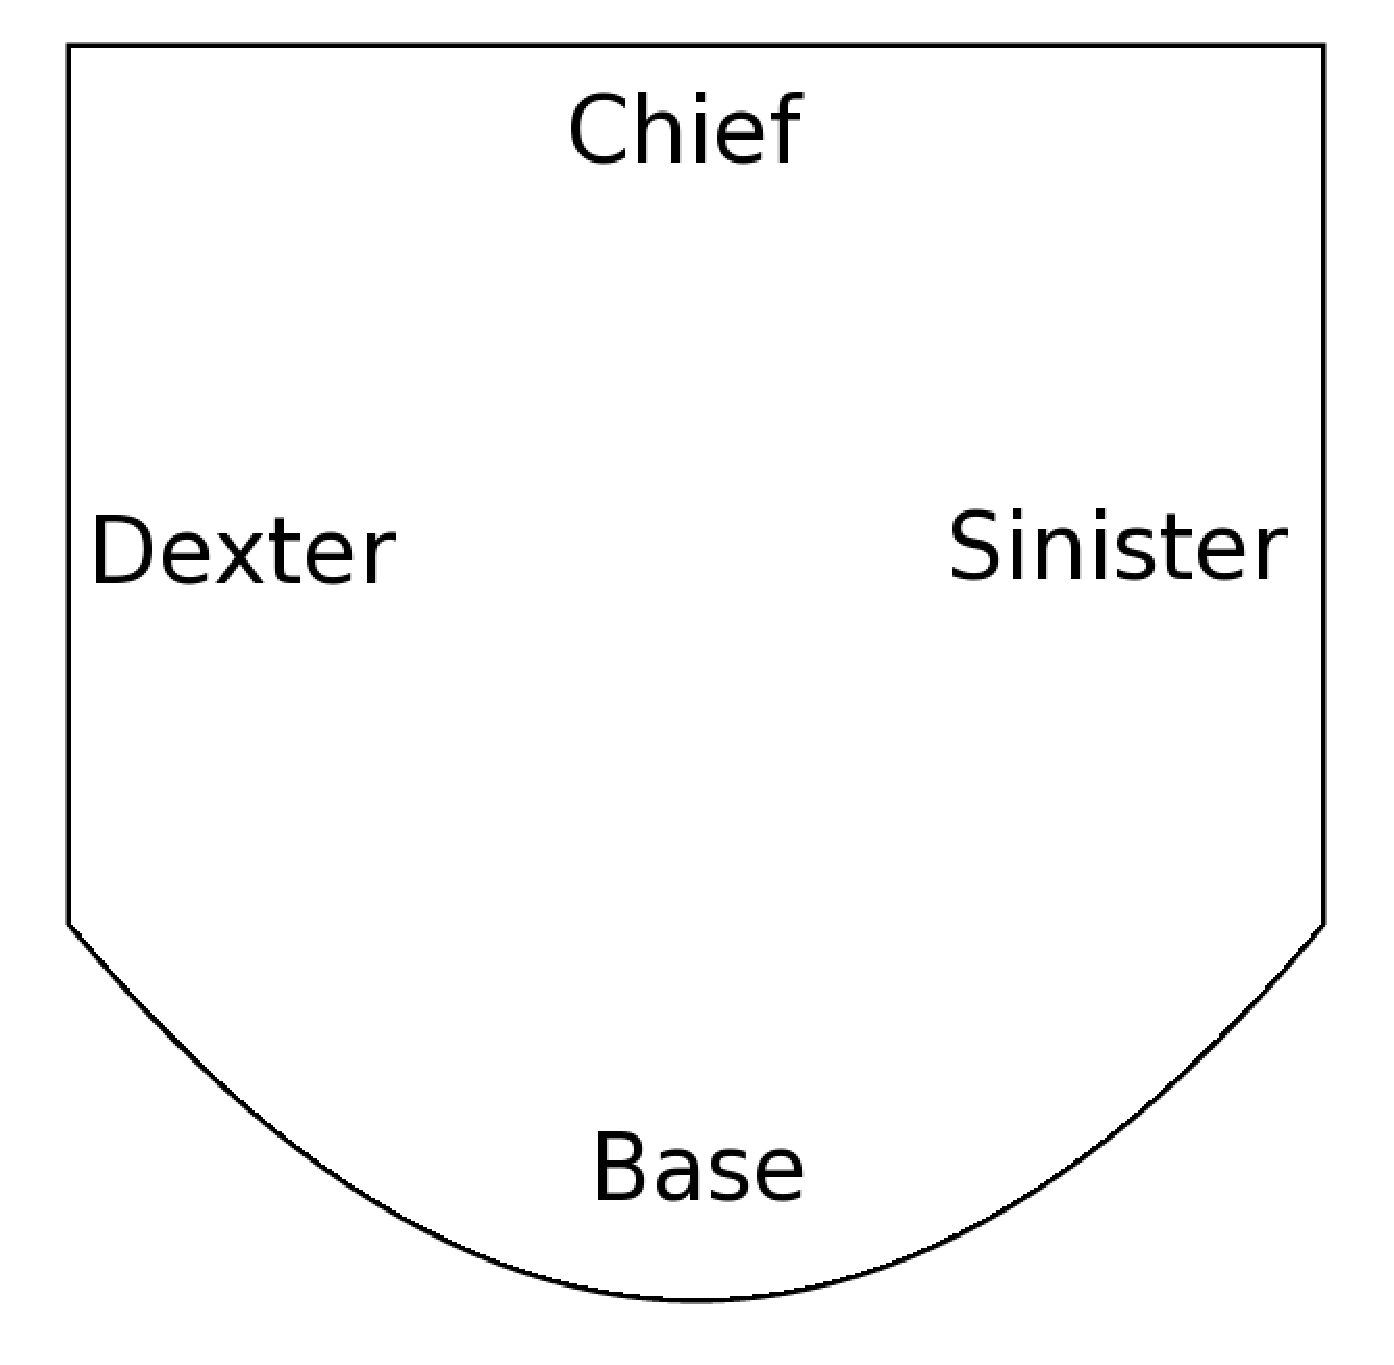
\includegraphics[width=0.6\textwidth]{Blazon/images/sides.eps}
  \caption{\emph{The sides of the field}}
  
\end{figure}

These keywords can be used to position Charges in a field relative to each other.  They can also be used to define direction, the most basic example of this is the Partition \emph{"Bend Sinister"} which is a diagonal line from lower left to upper right.
Semi-formal Charges can also be given a direction like so; \emph{"A Purse Fesswise Argent Spilling Coins to Dexter Argent"} which would depicts a purse lying horizontally with coins to the left hand side, from the viewers perspective.  

\begin{figure}[H]
  \centering
    
\includegraphics[width=0.6\textwidth]{Blazon/images/purse.eps}
  \caption{\emph{Per Bend Sinister Azure A Purse Fesswise Argent Spilling Coins to Dexter Argent Gules a Gauntlet Bendwise appaumy (an attitude meaning open palmed) Argent Bendwise sinister inverted proper.}\cite{fessways}}
  
\end{figure}



\section{Overall}
Blazon also encompasses a rudimentary system for layering.  Charges can be placed on top of the entire shield as long as the don't break the Rule of tincture of Obscure another Charge.  This is achieved with the keyword \emph{Overall} which occurs at the end of a Blazon sentence, when all the fields have been tinctured, and is then followed by a Charge. 


\section{Variations}
Finally Blazon has several pre-defined short hands for commonly used patterns known as variations.  These patterns are all achievable through sub-partitioning but in a very verbose manor.  \emph{"Checky Argent and Gules"} produces a silver and red grid pattern which for all intents and purposes is the same as placing a large number of \emph{Delfs} tinctured Gules onto a field tinctured Argent. 

By default Blazon will produce the pattern in quantities of six.  The number of repetitions can be stated by adding the suffix \emph{"of"} and then providing a quantity.  

\begin{figure}[H]
\subfigure[\emph{"Checky of eight Azure and Gules"}.]{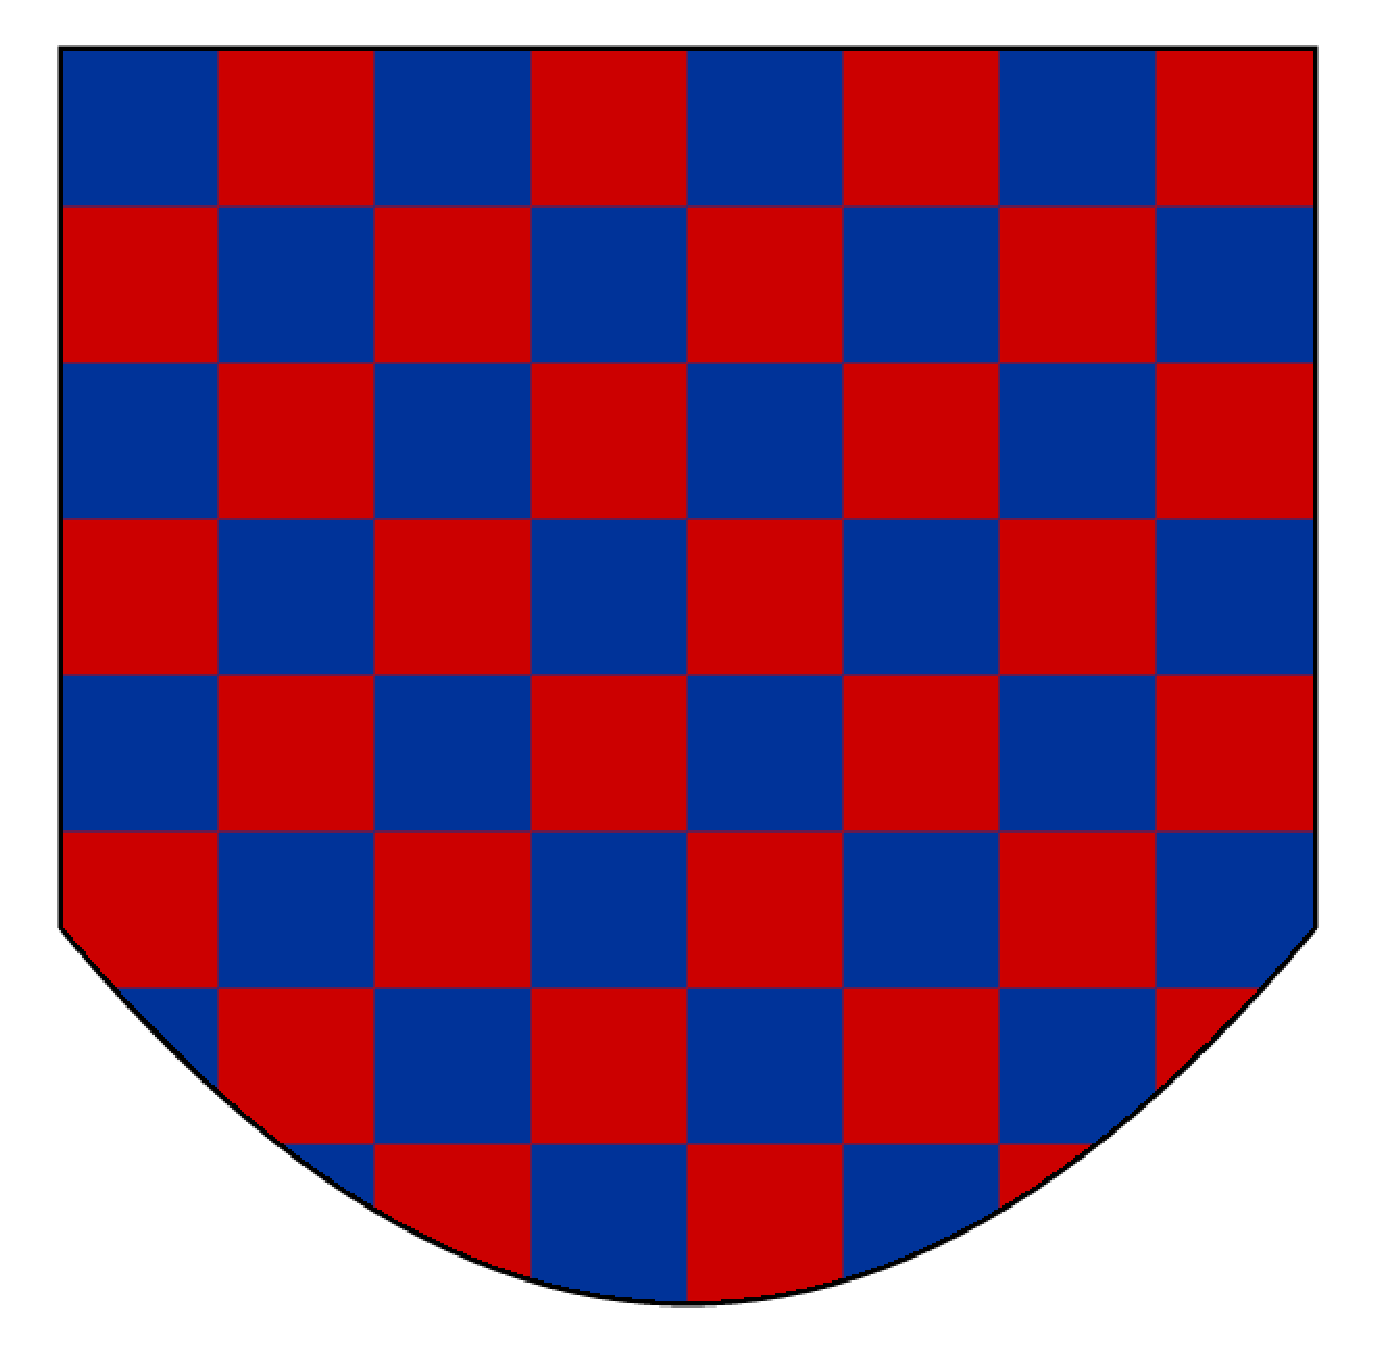
\includegraphics[width=0.5\textwidth]{Blazon/images/checky.eps}}
\hfill
\subfigure[\emph{"Paly of sixteen Sable and Or"}]{
\includegraphics[width=0.5\textwidth]{Blazon/images/paly.eps}}
\hfill

\caption{\emph{Two examples of short hand being used.}}

\end{figure}





%\begin{figure}[H]
%\subfigure[\emph{"A more complicated."}]{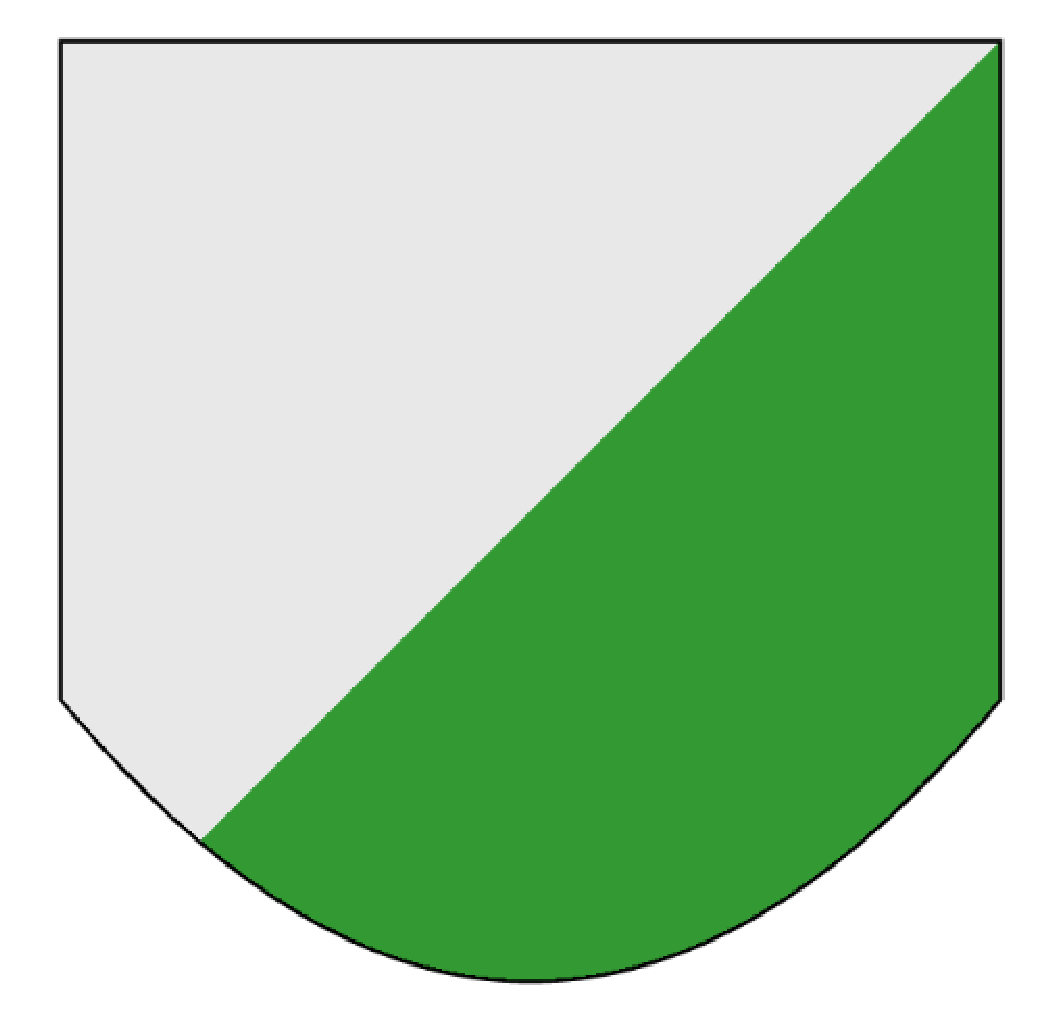
\includegraphics[width=0.4\textwidth]{Blazon/images/bendsinisterargentandvert.eps}}
%\hfill
%\caption{\emph{" "}.}
%\end{figure}